%%%% Dokumentklassen %%%%

\documentclass[a4paper,11pt,fleqn,dvipsnames,twoside,openany]{memoir} 	% Openright åbner kapitler på højresider (openany begge)

\usepackage{wrapfig}
%%%% PACKAGES %%%%
%% Oversættelse og tegnsætning %%
\usepackage[utf8]{inputenc}					% Input-indkodning af tegnsæt (UTF8)
\usepackage[danish]{babel}					% Dokumentets sprog
\usepackage[T1]{fontenc}					    % Output-indkodning af tegnsæt (T1)
\usepackage{ragged2e,anyfontsize}			% Justering af elementer
\usepackage{fixltx2e}						% Retter forskellige fejl i LaTeX-kernen
\usepackage{eso-pic}		
\newcommand\BackgroundPic{%
\put(0,0){%
\parbox[b][\paperheight]{\paperwidth}{%
\vfill
\centering
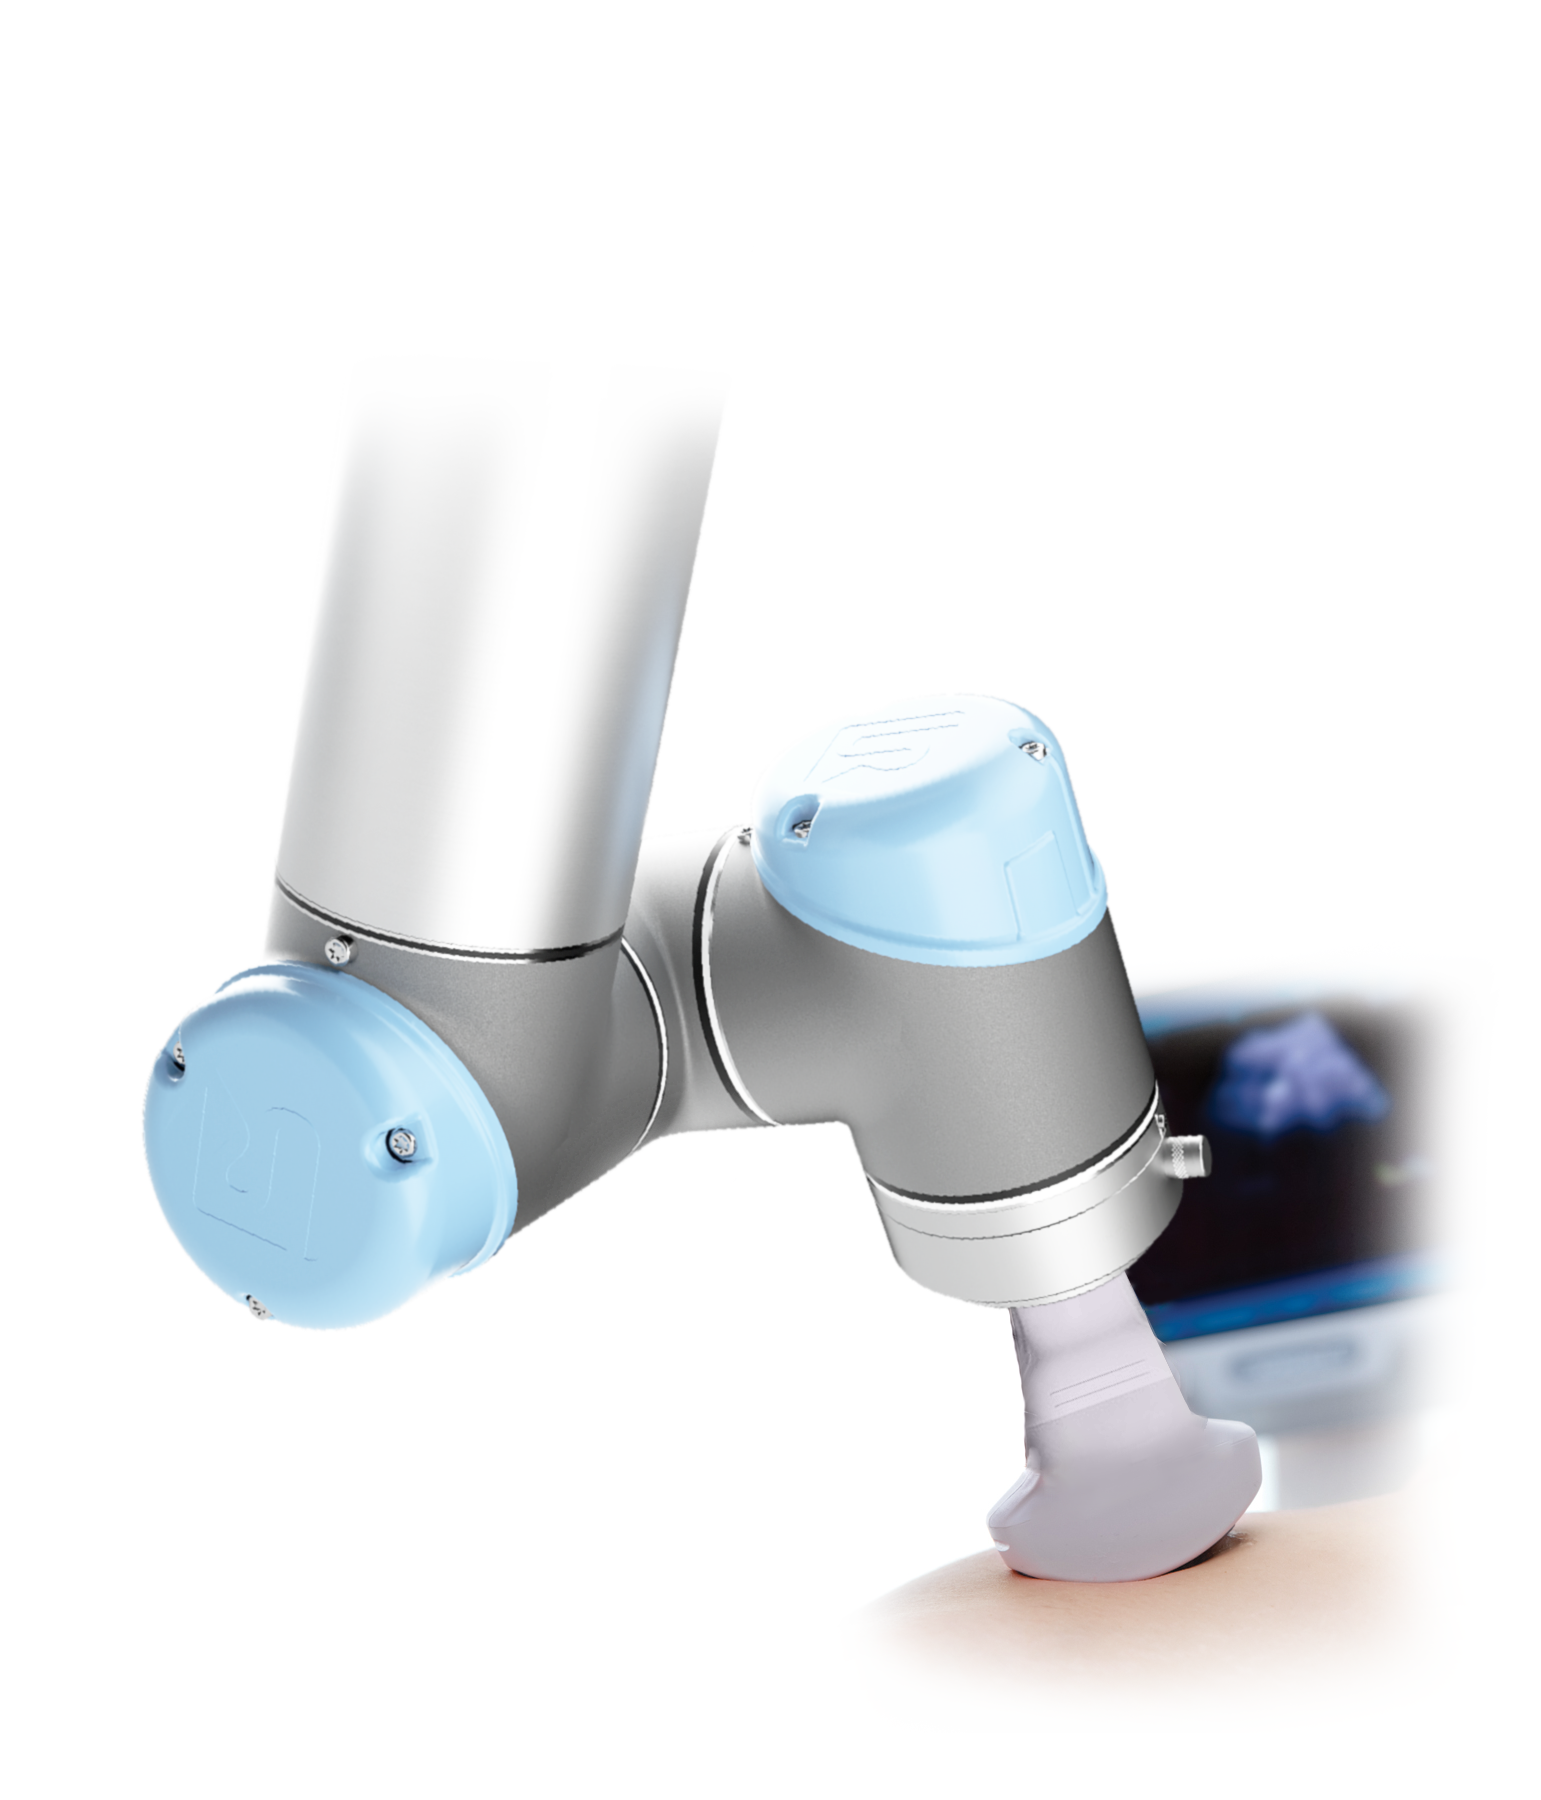
\includegraphics[width=\paperwidth,height=\paperheight,%
keepaspectratio]{figurer/forside.png}%
\vfill
}}}											
%% Figurer og tabeller (floats) %%
\usepackage{graphicx} 						% Håndtering af eksterne billeder (JPG, PNG, EPS, PDF)
\usepackage{multicol}         	            	% Muliggør output i spalter
\usepackage{rotating}						% Rotation af tekst med \begin{sideways}...\end{sideways}
\usepackage{xcolor}							% Definer farver med \definecolor. Se mere: http://en.wikibooks.org/wiki/LaTeX/Colors
\usepackage{flafter}						% Sørger for at floats ikke optræder i teksten før deres reference
\let\newfloat\relax 						% Justering mellem float-pakken og memoir
\usepackage{float}							% Muliggør eksakt placering af floats, f.eks. \begin{figure}[H]

%% Matematik mm. %%
\usepackage{amsmath,amssymb,stmaryrd} 		% Avancerede matematik-udvidelser
\usepackage{mathtools}						% Andre matematik- og tegnudvidelser
\usepackage{textcomp}                 		% Symbol-udvidelser (fx promille-tegn med \textperthousand)
\usepackage{rsphrase}						% Kemi-pakke til RS-saetninger, fx \rsphrase{R1}
\usepackage[version=3]{mhchem} 				% Kemi-pakke til flot og let notation af formler, f.eks. \ce{Fe2O3}
\usepackage{siunitx}						% Flot og konsistent præsentation af tal og enheder med \si{enhed} og \SI{tal}{enhed}
\sisetup{output-decimal-marker = {,}}		% Opsætning af \SI (DE for komma som decimalseparator) 
\usepackage{pdflscape}
\usepackage{afterpage}
%% Referencer og kilder %%
\usepackage[danish]{varioref}				% Muliggør bl.a. krydshenvisninger med sidetal (\vref)
\usepackage{natbib}							% Udvidelse med naturvidenskabelige citationsmodeller
\usepackage{xr}							    % Referencer til eksternt dokument med \externaldocument{<NAVN>}

%% Misc. %%
\usepackage{listings}						% Placer kildekode i dokumentet med \begin{lstlisting}...\end{lstlisting}
\usepackage{lipsum}							% Dummy text \lipsum[..]
\usepackage[shortlabels]{enumitem}			% Muliggør enkelt konfiguration af lister
\usepackage{pdfpages}						% Gør det muligt at inkludere pdf-dokumenter med kommandoen \includepdf[pages={x-y}]{fil.pdf}	
\pdfoptionpdfminorversion=6					% Muliggør inkludering af pdf-dokumenter, af version 1.6 og højere
\pretolerance=2500 							% Justering af afstand mellem ord (højt tal, mindre orddeling og mere luft mellem ord)	
\usepackage{hyperref}
%%%% CUSTOM SETTINGS %%%%
%% Marginer %%
\setlrmarginsandblock{3.5cm}{2.5cm}{*}		% \setlrmarginsandblock{Indbinding}{Kant}{Ratio}
\setulmarginsandblock{2.5cm}{3.0cm}{*}		% \setulmarginsandblock{Top}{Bund}{Ratio}
\checkandfixthelayout 						% Oversætter værdier til brug for andre pakker

%% Afsnitsformatering %%
\setlength{\parindent}{0mm}           		% Størrelse af indryk
\setlength{\parskip}{3mm}          			% Afstand mellem afsnit ved brug af double Enter
\linespread{1,1}							% Linjeafstand

%% Indholdsfortegnelse %%
\setsecnumdepth{subsection}		 			% Dybden af nummererede overskrifter (part/chapter/section/subsection)
\maxsecnumdepth{subsection}					% Dokumentklassens grænse for nummereringsdybde
\settocdepth{subsection} 					% Dybden af indholdsfortegnelsen
		
%% Opsætning af listings %%
\definecolor{commentGreen}{RGB}{34,139,24}
\definecolor{stringPurple}{RGB}{208,76,239}

\lstset{language=Matlab,					    % Sprog
	basicstyle=\ttfamily\scriptsize,		    % Opsætning af teksten
	keywords={for,if,while,else,elseif,		% Nøgleord at fremhæve
			  end,break,return,case,
			  switch,function},
	keywordstyle=\color{blue},				% Opsætning af nøgleord
	commentstyle=\color{commentGreen},		% Opsætning af kommentarer
	stringstyle=\color{stringPurple},		% Opsætning af strenge
	showstringspaces=false,					% Mellemrum i strenge enten vist eller blanke
	numbers=left, numberstyle=\tiny,		    % Linjenumre
	extendedchars=true, 					    % Tillader specielle karakterer
	columns=flexible,						% Kolonnejustering
	breaklines, breakatwhitespace=true,		% Bryd lange linjer
}

%% Navngivning %%
\addto\captionsdanish{
	\renewcommand\appendixname{Appendiks}
	\renewcommand\contentsname{Indholdsfortegnelse}	
	\renewcommand\appendixpagename{Appendiks}
	\renewcommand\appendixtocname{Appendiks}
	\renewcommand\cftchaptername{\chaptername~}		% Skriver "Kapitel" foran kapitlerne i indholdsfortegnelsen
	\renewcommand\cftappendixname{\appendixname~}	% Skriver "Appendiks" foran appendiks i indholdsfortegnelsen
}

%% Kapiteludssende %%
\definecolor{numbercolor}{gray}{0.7}		            % Definerer en farve til brug til kapiteludseende
\newif\ifchapternonum

\makechapterstyle{jenor}{					        % Definerer kapiteludseende frem til ...
  \renewcommand\beforechapskip{0pt}
  \renewcommand\printchaptername{}
  \renewcommand\printchapternum{}
  \renewcommand\printchapternonum{\chapternonumtrue}
  \renewcommand\chaptitlefont{\fontfamily{pbk}\fontseries{db}\fontshape{n}\fontsize{25}{35}\selectfont\raggedleft}
  \renewcommand\chapnumfont{\fontfamily{pbk}\fontseries{m}\fontshape{n}\fontsize{1in}{0in}\selectfont\color{numbercolor}}
  \renewcommand\printchaptertitle[1]{%
    \noindent
    \ifchapternonum
    \begin{tabularx}{\textwidth}{X}
    {\let\\\newline\chaptitlefont ##1\par} 
    \end{tabularx}
    \par\vskip-2.5mm\hrule
    \else
    \begin{tabularx}{\textwidth}{Xl}
    {\parbox[b]{\linewidth}{\chaptitlefont ##1}} & \raisebox{-15pt}{\chapnumfont \thechapter}
    \end{tabularx}
    \par\vskip2mm\hrule
    \fi
  }
}											        % ... her

\chapterstyle{jenor}						        % Valg af kapiteludseende - Google 'memoir chapter styles' for alternativer

%% Sidehoved %%

\makepagestyle{AAU}							        % Definerer sidehoved og sidefod udseende frem til ...
\makepsmarks{AAU}{%
	\createmark{chapter}{left}{shownumber}{}{. \ }
	\createmark{section}{right}{shownumber}{}{. \ }
	\createplainmark{toc}{both}{\contentsname}
	\createplainmark{lof}{both}{\listfigurename}
	\createplainmark{lot}{both}{\listtablename}
	\createplainmark{bib}{both}{\bibname}
	\createplainmark{index}{both}{\indexname}
	\createplainmark{glossary}{both}{\glossaryname}
}
\nouppercaseheads									% Ingen Caps ønskes

\makeevenhead{AAU}{\small BAC7 Automatisk Ultralydsscanner}{}{\leftmark}	% Definerer lige siders sidehoved (\makeevenhead{Navn}{Venstre}{Center}{Hoejre})
\makeoddhead{AAU}{\rightmark}{}{\small ASE}		            % Definerer ulige siders sidehoved (\makeoddhead{Navn}{Venstre}{Center}{Højre})
\makeevenfoot{AAU}{\small \thepage}{}{}						% Definerer lige siders sidefod (\makeevenfoot{Navn}{Venstre}{Center}{Højre})
\makeoddfoot{AAU}{}{}{\small \thepage}						% Definerer ulige siders sidefod (\makeoddfoot{Navn}{Venstre}{Center}{Højre})

\copypagestyle{AAUchap}{AAU}							% Sidehoved for kapitelsider defineres som standardsider, men med blank sidehoved
\makeoddhead{AAUchap}{}{}{}
\makeevenhead{AAUchap}{}{}{}
\makeheadrule{AAUchap}{\textwidth}{0pt}
\aliaspagestyle{chapter}{AAUchap}					% Den ny style vælges til at gælde for chapters
													% ... her
															
\pagestyle{AAU}										% Valg af sidehoved og sidefod


%%%% CUSTOM COMMANDS %%%%

%% Billede hack %%
\newcommand{\figur}[4]{
		\begin{figure}[H] \centering
			\includegraphics[width=#1\textwidth]{billeder/#2}
			\caption{#3}\label{#4}
		\end{figure} 
}

%% Specielle tegn %%
\newcommand{\decC}{^{\circ}\text{C}}
\newcommand{\dec}{^{\circ}}
\newcommand{\m}{\cdot}


%%%% ORDDELING %%%%

\hyphenation{mmHg}    %% Her kan defineres ordelingen for specifikke ord med "-". De forskellige ord adskilles med mellemrum. Fx \hyphenation{er-hvervs-liv-et Himmelstrup ka-kao}. I de fleste tilfælde kan LaTeX selv stå for det.

%%%% Tilføjelser af min preample %%%%

% Booktabs:
% The booktabs package is needed for better looking tables. 
\usepackage{booktabs}

% Caption:
% For better looking captions. See caption documentation on how to change the format of the captions.
\usepackage[hang, font={small, it}]{caption}

% Hyperref:
% This package makes all references within your document clickable. By default, these references will become boxed and colored. This is turned back to normal with the \hypersetup command below.
\usepackage{hyperref}
	\hypersetup{colorlinks=false,pdfborder=0 0 0}

% Cleveref:
% This package automatically detects the type of reference (equation, table, etc.) when the \cref{} command is used. It then adds a word in front of the reference, i.e. Fig. in front of a reference to a figure. With the \crefname{}{}{} command, these words may be changed.
\usepackage{cleveref}
	\crefname{equation}{formel}{formler}
	\crefname{figure}{figur}{figurer}	
	\crefname{table}{tabel}{tabeller}
	\crefname{section}{afsnit}{afsnit}
	\crefname{chapter}{kapitel}{kapitler}

% Mine tilføjelser:
\usepackage{nameref}                      %% Bruges til at kunne referere til kapitler og afsnits navne.
\usepackage{units}                        %% Bruges til at gøre fx 1/2 samlet med: \nicefrac{1}{2}.
\usepackage{tabu, longtable}              %% Bruges til tabeller.
\setlength{\tabulinesep}{2ex}             %% Definerer linjeafstand i tabeller.
\usepackage{enumerate}                    %% Bruges til lister.
\usepackage{tabto}                        %% Giver mulighed for TAB med fx \tabto{3em}.
\usepackage[hyphenbreaks]{breakurl}       %% Bruges til websiders url'er.
\renewcommand{\UrlFont}{                  %% Definerer url-font.
\small\ttfamily}                          %
\bibliographystyle{plain}                 %% Definere bibliografien. Ses til sidst i dokumentet i kapitlet Litteratur.
\usepackage[explicit]{titlesec}
\usepackage{longtable,tabu}
\usepackage{longtable}
\usepackage{todonotes}
\presetkeys{todonotes}{inline}{}
\usepackage{caption}
\usepackage{subcaption}
\externaldocument{Bilagsliste}

\titlespacing\section{0pt}{12pt plus 4pt minus 2pt}{0pt plus 2pt minus 2pt}
\titlespacing\subsection{0pt}{12pt plus 4pt minus 2pt}{0pt plus 2pt minus 2pt}
\titlespacing\subsubsection{0pt}{12pt plus 4pt minus 2pt}{0pt plus 2pt minus 2pt}
\raggedbottom
\begin{document}

\begin{titlingpage}
\begin{center}

~ \\[3cm]


\includegraphics[width=0.6\textwidth]{figurer/ASE}~\\[1cm]

\textsc{\LARGE Aarhus School of Engineering}\\[1.5cm]

\textsc{\Large Sundhedsteknologi og Informations- og kommunikationsteknologi}\\

\textsc{\Large Bachelorprojekt}\\[0.5cm]
\textsc{\Large Automatisk Ultralydsscanner} \\[1cm]

\noindent\makebox[\linewidth]{\rule{\textwidth}{0.4pt}}\\
[0.5cm]{\Huge Kravspecifikation}
\noindent\makebox[\linewidth]{\rule{\textwidth}{0.4pt}}

\end{center}

Charlotte Søgaard Kristensen (201371015) \newline
Mathias Siig Nørregaard  (201270810)\newline		 
Marie Kirkegaard (201370526) \newline  


\textit{Vejleder} \newline
Associate Professor\\
Michael Alrøe\\
Aarhus School of Engineering


\vfill

\begin{center}
{\large \today}
\end{center}

\end{titlingpage}

\tableofcontents

% Her findes de nummererede kapitler modsat \frontmatter og \backmatter.
%\chapter{Forkortelser}

\begin{table}[htb]
\centering
\begin{tabular}{ | c | p{0.80\textwidth} | }
\hline
\textbf{Forkortelser} & \textbf{Forklaring} \\\hline
ASE & Aarhus School of Engineering \\\hline
BDD & Block Definition Diagram \\\hline
FURPS+ & Funkctionality, Usability, Reliability, Performance, Supportability and Ekstra \\\hline
GUI & Graphical User Interface, Grafisk brugergrænseflade \\\hline
IBD & Internal Block Diagram \\\hline
MDD & Medical Device Directive \\\hline
MoSCoW & Must, Should, Could and Would like \\\hline
QALY & Kvalitet justeret leveår  \\\hline
RCT & randomized controlled trial \\\hline
SysML & Systems Modeling Language \\\hline
UC & Use case \\\hline
UML & Unified Modeling Language \\\hline

\end{tabular}
\caption{Forkortelser}
\end{table}

\vspace{3cm}
\chapter{Versionshistorik}\label{Versionshistorik}

\begin{table}[htb]
\begin{tabular}{ | l | l | l | p{0.49\textwidth} | }
\hline
\textbf{Version} & \textbf{Dato} & \textbf{Ansvarlig} & \textbf{Beskrivelse} \\\hline
1.0 & 2016-11-01 & CSK & Første version af udviklingsdokuement med systembeskrivelse, bdd og ibd\\\hline
1.1 & 2016-11-03 & CSK & Sekvensdiagrammer tilføjet  \\\hline
1.2 & 2016-11-04 & CSK, MSK & Forklaringer til sekvens- og klassediagrammer \\\hline
\end{tabular}
\caption{Versionshistorik}
\end{table}
\chapter{Indledning}\label{Formal}
Formålet med kravspecifikationen er at give kunden et detaljeret overblik over systemets funktionelle og ikke-funktionelle krav. Kravspecifikationen kan kaldes kontrakten mellem kunden og producenten af systemet. Forkortelser findes i bilag \ref{Satningsliste} Sætningsliste. 
\chapter{Systembeskrivelse}\label{Systembeskrivelse}
Formålet med Automatisk Ultralydsscanner er at gøre det muligt at lave en fuldautomatisk ultralydsscanninger af mamma til screening for brystkræft. En operatør med kendskab til ultralyd kan via en grafisk brugergrænseflade (GUI) betjene systemet, bestående af en PC Applikation installeret på en computer. Operatøren skal tænde for robotarmen og sikre, at 3D kamera er tilsluttet til computeren gennem 3D kameraets USB-kabel. Operatøren sikrer forbindelsen til robotarmen med et access point. Robotarmen er tilsluttet til access pointet gennem et ethernetkabel, og videre til computeren gennem et andet ethernetkabel fra access point til computeren.  

Robotarmen har på det yderste led påmonteret en ultralydsprobe, og robotarmen er placeret ved siden af briksen, hvor patienten skal ligge. 3D kameraet er monteret i loftet over briksen. Operatør guider patienten til at ligge på briksen og sikrer, at  brystområdet er indenfor intervallet og hovedet er udenfor intervallet. 

Operatør sørger for, at ultralydsscanneren er tændt, og gennem PC Applikation har operatøren mulighed for at 3D scanne en patients brystområde. PC Applikation processerer brystområdets form og position fra 3D kameraet og leverer informationen videre til robotarmen, som fører ultralysdsproben fra ultralydsscanneren rundt på brystområdet.  Operatøren kan følge med på ultralydsscannerens skærm under scanningen. 

Figur \ref{Systembeskrivelse} viser en oversigt over systemet og interaktionen mellem aktørerne. 

\begin{figure}[H]
    \centering
    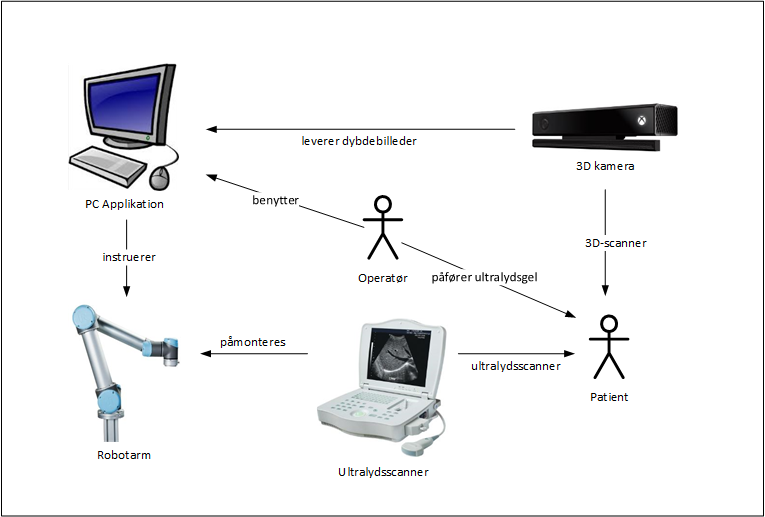
\includegraphics[width=0.67\textwidth]{figurer/d/Kravspecifikation/Systembeskrivelse}
    \caption{Systemoversigt}
    \label{Systembeskrivelse}
\end{figure}
\pagebreak

\chapter{Aktører}\label{Aktorer}

Aktørerne kan enten påvirke eller blive påvirket af systemet. Primære aktører er interessenter, der kalder på systemet til at levere service, mens sekundære aktører leverer en service til systemet. 

Tabel \ref{Beskriv} viser aktørbeskrivelser, og hvordan hver aktør interagerer med Automatisk Ultralydsscanner. 

\section{Aktørbeskrivelse}
\begin{table}[htb]
\begin{tabular}{|l|l|p{0.6\textwidth}| }
  \hline
  \textbf{Aktørnavn} & \textbf{Type} & \textbf{Beskrivelse} \\ \hline
  Operatør & Primær & Operatør betjener Automatisk Ultralydsscanner 
  \\ \hline
  Patient & Sekundær & Patient er personen, hvorpå scanningen foregår \\ \hline
  Robotarm & Sekundær & Robotarm styrer Ultralydsscanner i det detekterede brystområde \\ \hline
Ultralydsscanner & Sekundær & Ultralydsscanner danner ultralydsvideoclips, som Operatør kan følge på Ultralydsscanners skærm\\ \hline
  3D kamera & Sekundær & 3D kamera scanner det brystområde, hvorpå Ultralydsscanner skal foretage scanning \\ \hline 
\end{tabular}
\caption{Aktørbeskrivelse}
\label{Beskriv}
\end{table}
\newpage

\subsection{Aktør-kontekst diagram}
I figur \ref{akDiagram} ses et aktør-kontekst diagram, som viser interaktionen mellem aktørerne og PC Applikation. Primære aktører er afbilledet på venstre side og de sekundære er afbilledet på højre side.

\begin{figure}[H]
    \centering
    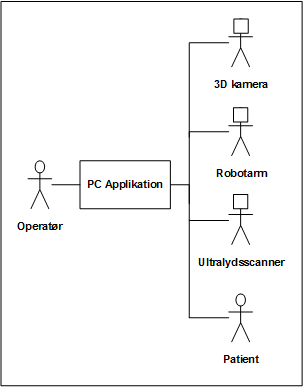
\includegraphics[width=0.70\textwidth]{figurer/d/Kravspecifikation/uml_aktor}
    \caption{Aktør-kontekstdiagram.}
    \label{akDiagram}
\end{figure}
\chapter{Funktionelle krav}\label{Funktionellekrav}
De funktionelle krav beskriver de funktioner, systemet skal have. Kravene er beskrevet ved hjælp af use cases, der bl.a. beskriver, hvordan en aktører anvender systemet til at opnå et mål. Figur \ref{UseCaseDiagram} viser et use case diagram, som illustrerer den enkeltes aktørs interaktion med de de forskellige use cases. 

\section{Use Case Diagram}
\begin{figure}[H]
    \centering
    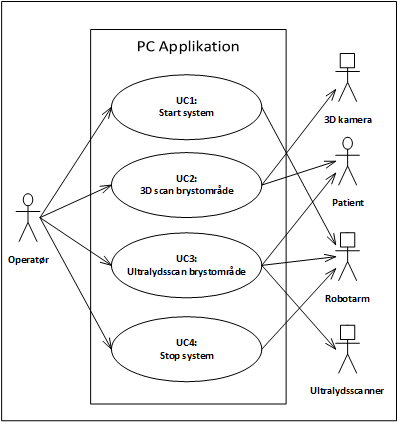
\includegraphics[width=0.80\textwidth]{figurer/d/Kravspecifikation/UseCaseDiagram}
    \caption{Use Case Diagram}
    \label{UseCaseDiagram}
\end{figure}
\newpage

\section{Fully-dressed Use Cases}
Hver use case (UC) er beskrevet med et mål, interagerende aktører, hvad der initerer use casen, forudsætningen, resultat og forløbet i use casen. Målet beskriver, hvad der ønskes opnået, mens resultatet beskriver, hvad systemet har gjort ved slutningen af use casen. 

Efter afsluttelse af UC1: Start system, vil det til en hver tid være muligt at afbryde den igangværende use case, og dermed starte UC4: Stop system.

\subsection{Use Case 1}
\begin{longtabu}{ | l | p{0.8\textwidth} | }
  \hline
  \multicolumn{2}{|c|}{\textbf{UC1: Start system}} \\ \hline
  \textbf{Mål} & At forberede scanninngen \\ \hline
  \textbf{Aktører} & Operatør, Robotarm \\ \hline
  \textbf{Initiering} & Operatør  \\ \hline
  \textbf{Forudsætninger} & Computer, der skal køre PC Applikation, er tændt. Robotarm er tilsluttet  \\ \hline
  \textbf{Resultat} & PC Applikation er startet \\ \hline
  \textbf{Hovedforløb} & 
  	{\begin{enumerate}
  	\item Operatør starter PC Applikation ved at klikke på 'AutoSonography.exe' på computerens skrivebord
  	\item PC Applikation instruerer Robotarm tilbage til standardposition
  	\end{enumerate}} \\\hline
\end{longtabu}
\newpage

\subsection{Use Case 2}
\begin{longtabu}{ | l | p{0.8\textwidth} | }
  \hline
  \multicolumn{2}{|c|}{\textbf{UC2: 3D scan brystområde}} \\\hline
  \textbf{Mål} & At konstruere et dybdebillede af Patients brystområde, så UC3: Ultralydsscan brystområde kan begyndes  \\\hline
   \textbf{Aktører} & Operatør, Patient, 3D kamera \\\hline
  \textbf{Initiering} & Operatør  \\\hline
  \textbf{Forudsætninger} & UC1: Start system  er gennemført. 3D kamera er tilsluttet computeren. Patients brystområde er indenfor afgræsning, mens Patients hoved og arme er udenfor afgrænsning \\\hline
  \textbf{Resultat} & Patients brystområde er blevet scannet af 3D kamera \\\hline
  \textbf{Hovedforløb} & 
  	{\begin{enumerate} 
  	\item Operatør trykker på knappen [3D Scan] på GUI's Startup Menu
  	\item Operatør trykker på knappen [Scan] på GUI's 3D Scan Menu
	\begin{itemize}
	\item \textit{'Juster 3D billedets skæring'}  	
  	\end{itemize} 
  	\item PC Applikation instruerer 3D kamera til at scanne brystområde på Patient
  	\item Operatør godkender dybdebilledet på knappen [OK] på GUI's 3D Scan Menu efter efter endt scanning 
	\begin{itemize}
	\item \textit{'Scanning er ikke godkendt'}  	
  	\end{itemize} 
  	\end{enumerate}} \\\hline
\textbf{Udvidelser} & 
  	{\begin{itemize} 
  	\item \textit{'Juster 3D billedets skæring'}
  		\begin{enumerate}[label=A\arabic*]
		\item Operatør vælger et andet skæringsinterval på GUI for Patients brystområde
		\item Operatør forsætter UC2: 3D scan brystområde i punkt 2   		
  		\end{enumerate}
  	\end{itemize}} \\ \hline
  \textbf{Undtagelser} & 
  	{\begin{itemize} 
  	\item \textit{'Scanning er ikke godkendt'}
  		\begin{enumerate}[label=B\arabic*]
  		\item Operatør godkender ikke dybdebilledet og går i udvidelsen 'Juster 3D billedets skæring'
  		\end{enumerate}
  	\end{itemize}} \\\hline
	\end{longtabu}
\newpage

\subsection{Use Case 3}
\begin{longtabu}{ | l | p{0.8\textwidth} | }
  \hline
  \multicolumn{2}{|c|}{\textbf{UC3: Ultralydsscan brystområde}} \\ \hline
  \textbf{Mål} & At få en ultralydsscanning af Patients brystområde \\ \hline
   \textbf{Aktører} & Operatør, Robotarm, Ultralydsscanner \\ \hline
  \textbf{Initiering} & Operatør \\ \hline
  \textbf{Forudsætninger} & UC2: 3D scan brystområde er gennemført. Patient har ikke skiftet position fra UC3: 3D scan brystområde.  Ultralydsscanner er tændt. Robotarm  er tændt og tilsluttet  \\ \hline
  \textbf{Resultat} & PC Applikation har instrueret Robotarm i at flytte Ultralydsscanner omkring Patients brystområde således, at der konstrueres en ultralydsscanning \\ \hline
  \textbf{Hovedforløb} & 
  	{\begin{enumerate} 
  	\item Operatør trykker på knappen [Ultralyddscan] på GUI's Startup Menu
  	\item PC Applikation benytter 3D kameras dybdebillede fra UC2: 3D scan brystområde til at instruere Robotarm til ny positur, for at bevæge Ultralydsscanner på Patient i et specifikt bevægelsesmønster (se kapitel \ref{Monster} Krav til specifikt bevægelsesmønster)
  	  	\begin{itemize}
  	  	\item \textit{'Operatør pauser scanning'}
  		\item \textit{'Operatør stopper scanning'}
  		\end{itemize}
  	\item PC Applikation instruerer Robotarm tilbage til standardposition
  	\end{enumerate}} \\ \hline
  	\textbf{Udvidelser} & 
  	{\begin{itemize} 
  	\item \textit{'Operatør pauser scanning'}
  		\begin{enumerate}[label=A\arabic*]
  		\item Operatør trykker på knappen [Pause] på GUI's Ultralydsscan Menu, og PC Applikation stopper Robotarm indenfor 5 sekunder
  		\item Operatør trykker på knappen [Pause] på GUI's Ultralydsscan Menu, og Robotarm genoptager scanningen indenfor 2 sekunder   		
  		\end{enumerate}
  	\end{itemize}} \\ \hline
  \textbf{Undtagelser} & 
  	{\begin{itemize} 
  	\item \textit{'Operatør stopper scanning'}
  		\begin{enumerate}[label=B\arabic*]
  		\item Operatør trykker på knappen [Stop] på GUI's Ultralydsscan Menu
  		\item PC Applikation instruerer Robotarm tilbage til standardposition
  		\end{enumerate}
  	\end{itemize}} \\\hline
\end{longtabu}

\subsection{Use Case 4}
\begin{longtabu}{ | l | p{0.8\textwidth} | }
  \hline
  \multicolumn{2}{|c|}{\textbf{UC4: Stop system}} \\ \hline
  \textbf{Mål} & At stoppe systemet \\ \hline
  \textbf{Aktører} & Operatør, Robotarm \\ \hline
  \textbf{Initiering} & Operatør\\ \hline
  \textbf{Forudsætninger} & UC1: Start system er færdiggjort. Robotarm  er tændt og tilsluttet  \\ \hline
  \textbf{Resultat} & PC Applikation er lukket ned og Robotarm er i standardposition\\ \hline	
  \textbf{Hovedforløb} & 
  	{\begin{enumerate}
  	\item Operatør lukker softwaren ved at trykke på knappen [Luk] på GUI's Startup Menu
  	\item PC Applikation instruerer Robotarm tilbage til standardposition
  	\end{enumerate}} \\ \hline
\end{longtabu}
\chapter{Ikke-funktionelle krav}\label{Ikkefunktionellekrav}

Ikke-funktionelle krav er begrænsninger til løsning af projektets funktionelle krav. Til at beskrive de ikke-funktionelle krav er MoSCoW og FURPS+ metoderne anvendt. 
MoSCoW-metoden betegner krav, som systemet skal opfylde (must), de krav som systemet bør realisere (should), de krav som systemet kunne realisere, men ikke har indvirkning på de andre krav (could), og de krav som omhandler fremtidige opdateringer og udvidelser eller krav som ikke implementeres  (would/won't).
  
FURPS+ står for:
\begin{enumerate}
\item[F.] Funktionelle krav, som er angivet i Use Cases.
\item[U.] Usability
\item[R.] Reliability
\item[P.] Performance 
\item[S.] Supportability 
\item[+.] Ekstra krav til systemet, som ikke hører ind under ovenstående. 
\end{enumerate}

%%%
\section{Usability}
\begin{enumerate}
    \item[U1.] PC Applikation skal have en GUI. (must)
    \item[U2.] Operatør bør kunne lære at ultralydsscanne Patient med Automatisk Ultralydsscanner på 2 timer. (should)
    \item[U3.] Systemet bør have en brugervejledning.  (should)  
    \item[U4.] Operatør, med kendskab til ultralyd, bør kunne betjene PC Applikation. (should)
    \item[U5.] PC Applikation bør kunne hente gamle målinger. (could)
\end{enumerate}

%%%
\section{Performance}
\begin{enumerate}
    \item[P1.] Scanning med 3D kamera og ultralydsscanning skal max tage 10 minutter til sammen. (must) 
    \item[P2.] Starttid på PC Applikation skal være max 10 sekunder. (must)
    \item[P3.] 3D kamera skal max bruge 10 sekunder på at tage 3D billedet. (must)
    \item[P4.] PC Applikation skal max bruge 10 sekunder på at færdiggøre brystområdets positurer til Robotarm. (must)
    \item[P5.] Robotarm bør have en tryksensor monteret. (should)
\end{enumerate}

%%%
\section{Supportability}
\begin{enumerate}
    \item[S1.] Ultralydsscanners probe bør kunne desinficeres med hospitalssprit. (should)
    \item[S2.] Operatør bør have mulighed for at skifte Ultralydsscanner til systemet. (should)
    \item[S3.] PC Applikation bør benytte n-tier architecture. (should)
    \item[S4.] Softwaren bør opbygges efter programmeringsprincipperne SOLID. (should)
\end{enumerate}
%%%
\section{Ekstra(+)}\label{andrePlus}

\begin{enumerate}
	\item[+1.] Systemet bør overholde Medical Device Directive 93/42/EØF \cite{MDD} (should)
	\item[+2.] PC Applikation bør overholde Standarden DS/EN 63204:2006 - Software for medicinsk udstyr - Livscyklusprocesser for software \cite{software} (should)
    \item[+3.] I fremtiden kan PC Applikation opdateres med en funktion, der lokaliserer og identificerer knuder. (would)
    \item[+4.] I fremtiden kan Operatør registrere en Patient i PC Applikation. (would) 
    \item[+5.] I fremtiden kan Operatør gemme og hente en måling i PC Applikation. (would)  
    \item[+6.] I fremtiden kan Operatør slette en måling i PC Applikation. (would)
    \item[+7.] I fremtiden kan PC Applikation have en database til at lagre data. (would)
    \item[+8.] I fremtiden kan Operatør tilgå PC Applikation gennem login. (would) 
    \item[+9.] I fremtiden kan Operatør identificere Patient i PC Applikation ud fra et patientidentifikation. (would)
\end{enumerate}

\chapter{Krav til specifikt bevægelsesmønster} \label{Monster}
Kravet om et specifikt bevægelsesmønster er lavet for at sikre, at hele brystet bliver scannet af Ultralydsscanner. Ved traditionelle scanninger, foretaget af radiologer, føres ultralydsproben i en sinus-lignende kurve med overlap, startende fra højre side af højre bryst til venstre side af højre bryst, og derefter fra højre side af venstre bryst ud til venstre side af venstre bryst. Det skal sikres, at ultralydsproben starter og slutter uden for brystvævet, hvilket sikrer, at hele brystet er scannet. Bevægelsesmønsteret er illustreret i Figur \ref{Probensbevagelse} nedenfor. 

\begin{figure}[H]
    \centering
    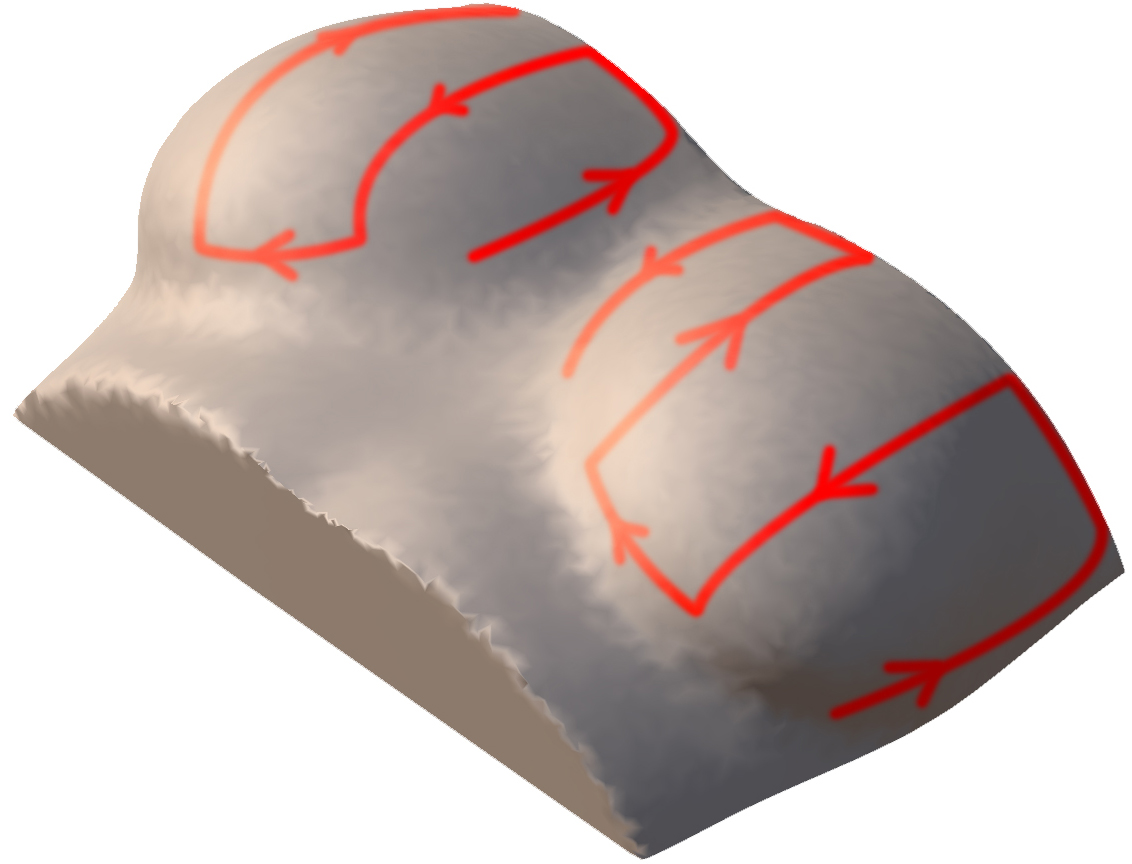
\includegraphics[width=0.75\textwidth]{figurer/d/probebevagelse}
    \caption{Probens bevægelsesbane på brystet}
    \label{Probensbevagelse}
\end{figure}

Bevægelsesmønsteret er bestemt ud fra interview med radiolog Lars Bolvig. For interview se bilag \ref{Telefoninterview} Interview med radiolog Lars Bolvig. 
\chapter{Brugergrænseflade}\label{Brugerganseflade}

PC Applikation til Automatisk Ultralydsscanner består af forskellige menuer.  Det er muligt for Operatør at betjene systemet gennem PC Applikations GUI ved tryk på forskellige knapper i menuerne. 

\section{Menuer}
Nedenstående beskriver PC Applikations forskellige menuer. 
\begin{itemize}
\item \textbf{Startup Menu:} Operatør præsenteres for denne menu ved opstart af PC Applikation, hvor Operatør har mulighed for at vælge en 3D scanning. Efter en 3D scanning vil Operatør kunne vælge enten at lave en ny 3D scanning eller ultralydsscanning. 
\item \textbf{3D Scan Menu: } Operatør bliver præsenteret for 3D kameras scanningsområde, hvor Operatør kan justere, så brystområdet er indenfor intervallet. Efter scanning vil der vises en 3D model af brystet. 
\item \textbf{Ultralydsscan Menu:} Operatør har mulighed for at pause eller stoppe scanning. 
\end{itemize}

\section{Knapper}
Nedenstående beskriver PC Applikations forskellige knapper. 
\begin{itemize}
\item \textbf{Luk Knap:} Findes på samtlige menuer øverst i højre hjørne. Et tryk på knappen vil lukke PC Applikation ned. 
\item \textbf{3D Scan Knap:} Findes på menuen 'Startup Menu'. Et tryk på knappen vil åbne menuen '3D Scan Menu'. 
\item \textbf{Ultralydsscan Knap:} Findes på menuen 'Startup Menu'. Et tryk på knappen vil åbne menuen 'Ultralydsscan Menu' og påbegynde 'UC3: Ultralydsscan'. 
\item \textbf{Scan Knap:} Findes på menuen '3D Scan Menu'. Et tryk på knappen vil påbegynde 3D 'UC2: 3D scan'. 
\item \textbf{OK Knap:} Findes på menuen '3D Scan Menu'. Et tryk på knappen vil åbne menuen 'Startup Menu'. 
\item \textbf{Pause Knap:} Findes på menuen 'Ultraldydsscan Menu'. Et tryk på knappen vil midlertidigt pause scanning.  
\item \textbf{Resume Knap:} Findes på menuen 'Ultraldydsscan Menu'. Et tryk på knappen vil genoptage scanning efter den er pauset. 
\item \textbf{Stop Knap:} Findes på menuen 'Ultralydsscan Menu'. Et tryk på knappen vil afslutte ultralydsscanningen. 
\end{itemize}

\section{Track bars}
Nedenstående beskriver PC Applikations '3D Scan Menu' track bars til afgrænsning af brystområdet.  
\begin{itemize}
\item \textbf{Y Min:} Denne track bar justerer den røde streg på GUI, som skal være under brystet på Patient. 
\item \textbf{Y Max:} Denne track bar justerer den blå streg på GUI, som skal være over brystet på Patient. 
\end{itemize}

\section{Skitser}
Nedenstående figurer er skitser af de forskellige menuer i PC Applikation. 

\begin{figure} [h]
    \centering
    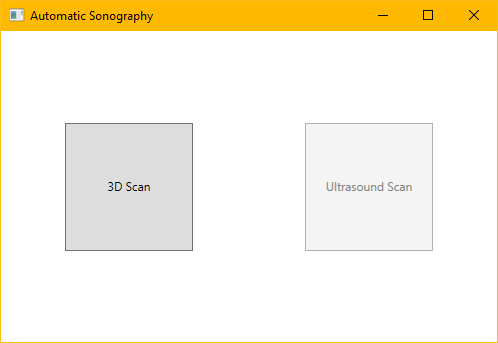
\includegraphics[width=0.9\textwidth]{figurer/d/GUIskitse/main_menu}
    \caption{3D Scan menu}
    \label{3Dscan}
\end{figure}

\begin{figure} [h]
    \centering
    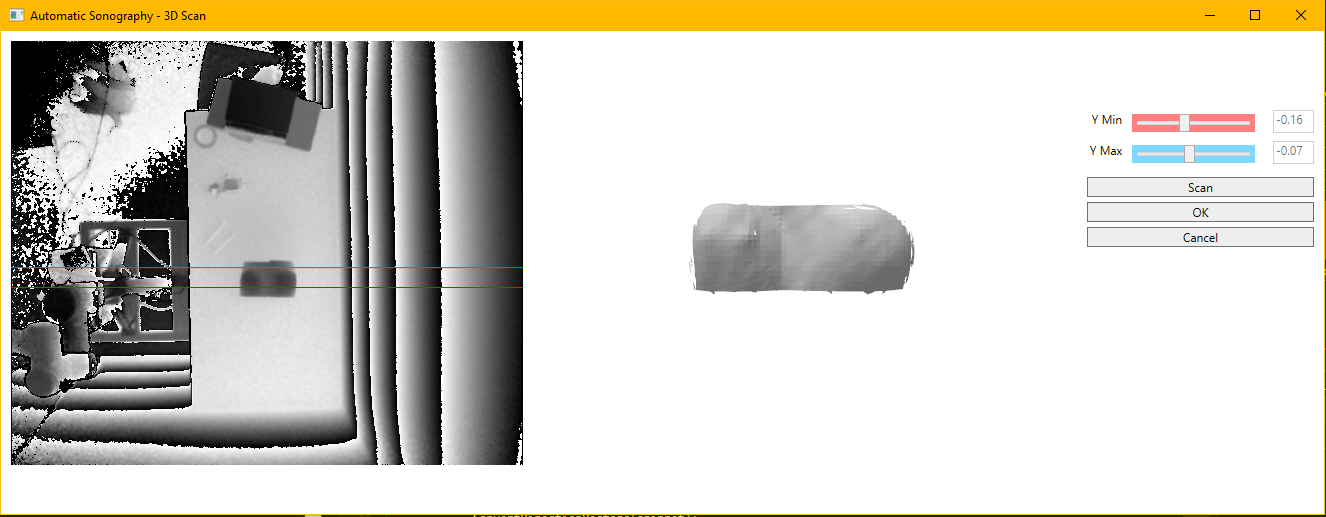
\includegraphics[width=0.9\textwidth]{figurer/d/GUIskitse/3d_scan}
    \caption{3D Scan menu}
    \label{3Dscan}
\end{figure}

\begin{figure}[h]
    \centering
    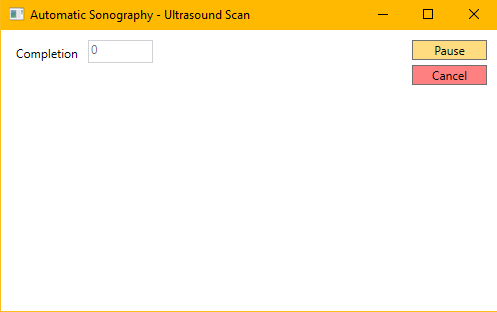
\includegraphics[width=0.9\textwidth]{figurer/d/GUIskitse/ultrasound_scan}
    \caption{Ultralydsscan menu}
    \label{Ultralydsscan}
\end{figure}

\backmatter
\chapter{Bilag}\label{Bilag}

\ref{Satningsliste} Sætningsliste \\
\ref{UR10spec} UR10 Specifikation \\
%\refl{UserManualUR10}


\bibliographystyle{plain}
\bibliography{bibliografi/PRJ3}    % Sætter bibliografien bagerst i dokumentet. Bruger bib-filen PRJ3.

\end{document}
